% --------------------------------------------------------------
% This is all preamble stuff that you don't have to worry about.
% Head down to where it says "Start here"
% --------------------------------------------------------------
 
\documentclass[addpoints,12pt,answers]{exam}
\usepackage[utf8]{inputenc}
\usepackage{parskip}
\usepackage{color}
\usepackage{graphicx}
\usepackage[normalem]{ulem}

\definecolor{mycrimson}{cmyk}{0.25,1,.79,.20}
\CorrectChoiceEmphasis{\color{mycrimson}\bfseries}

\title{Lecture Exercise \#2: Equipment Calculations (34pts)}
\author{Dr. Armen Amirkhanian, P.E.\\CE461/561--Horizontal Construction}
\date{Due: September 13, 2018}

\begin{document}

\maketitle

\begin{center}
\fbox{\fbox{\parbox{5.5in}{
\vspace{0.1in}
\textbf{By submitting this assignment on Blackboard, you acknowledge that you understand the UA Academic Honor Code. You promise or affirm that you will not at any time be involved with cheating, plagiarism, fabrication or misrepresentation while enrolled as a student at The University of Alabama. You agree that you have read the Academic Honor Code, which explains disciplinary procedures that will result from the aforementioned. You understand that violation of this code will result in penalties as severe as indefinite suspension from the University.
\vspace{0.1in}}}}}
\end{center}

\newpage
\begin{questions}
\question[8] Your lab technician has run a bunch of soil density tests for your jobsite but is on Reddit so much that the density curve never got calculated. Using the values available in the data file on Blackboard, perform the appropriate calculations to obtain and graph the moisture density curve for the two aggregate sources (Cray Court and Hanson Jeff). Make a separate chart for each aggregate source. Indicate the OMC and maximum dry density on the chart. Also, indicate somewhere on the chart (i.e. textbox) what the AASHTO group classification is of the soil. An example chart is shown below (yours will not look exactly like this, do not use this chart as a check against your calculations!). 
\begin{center}
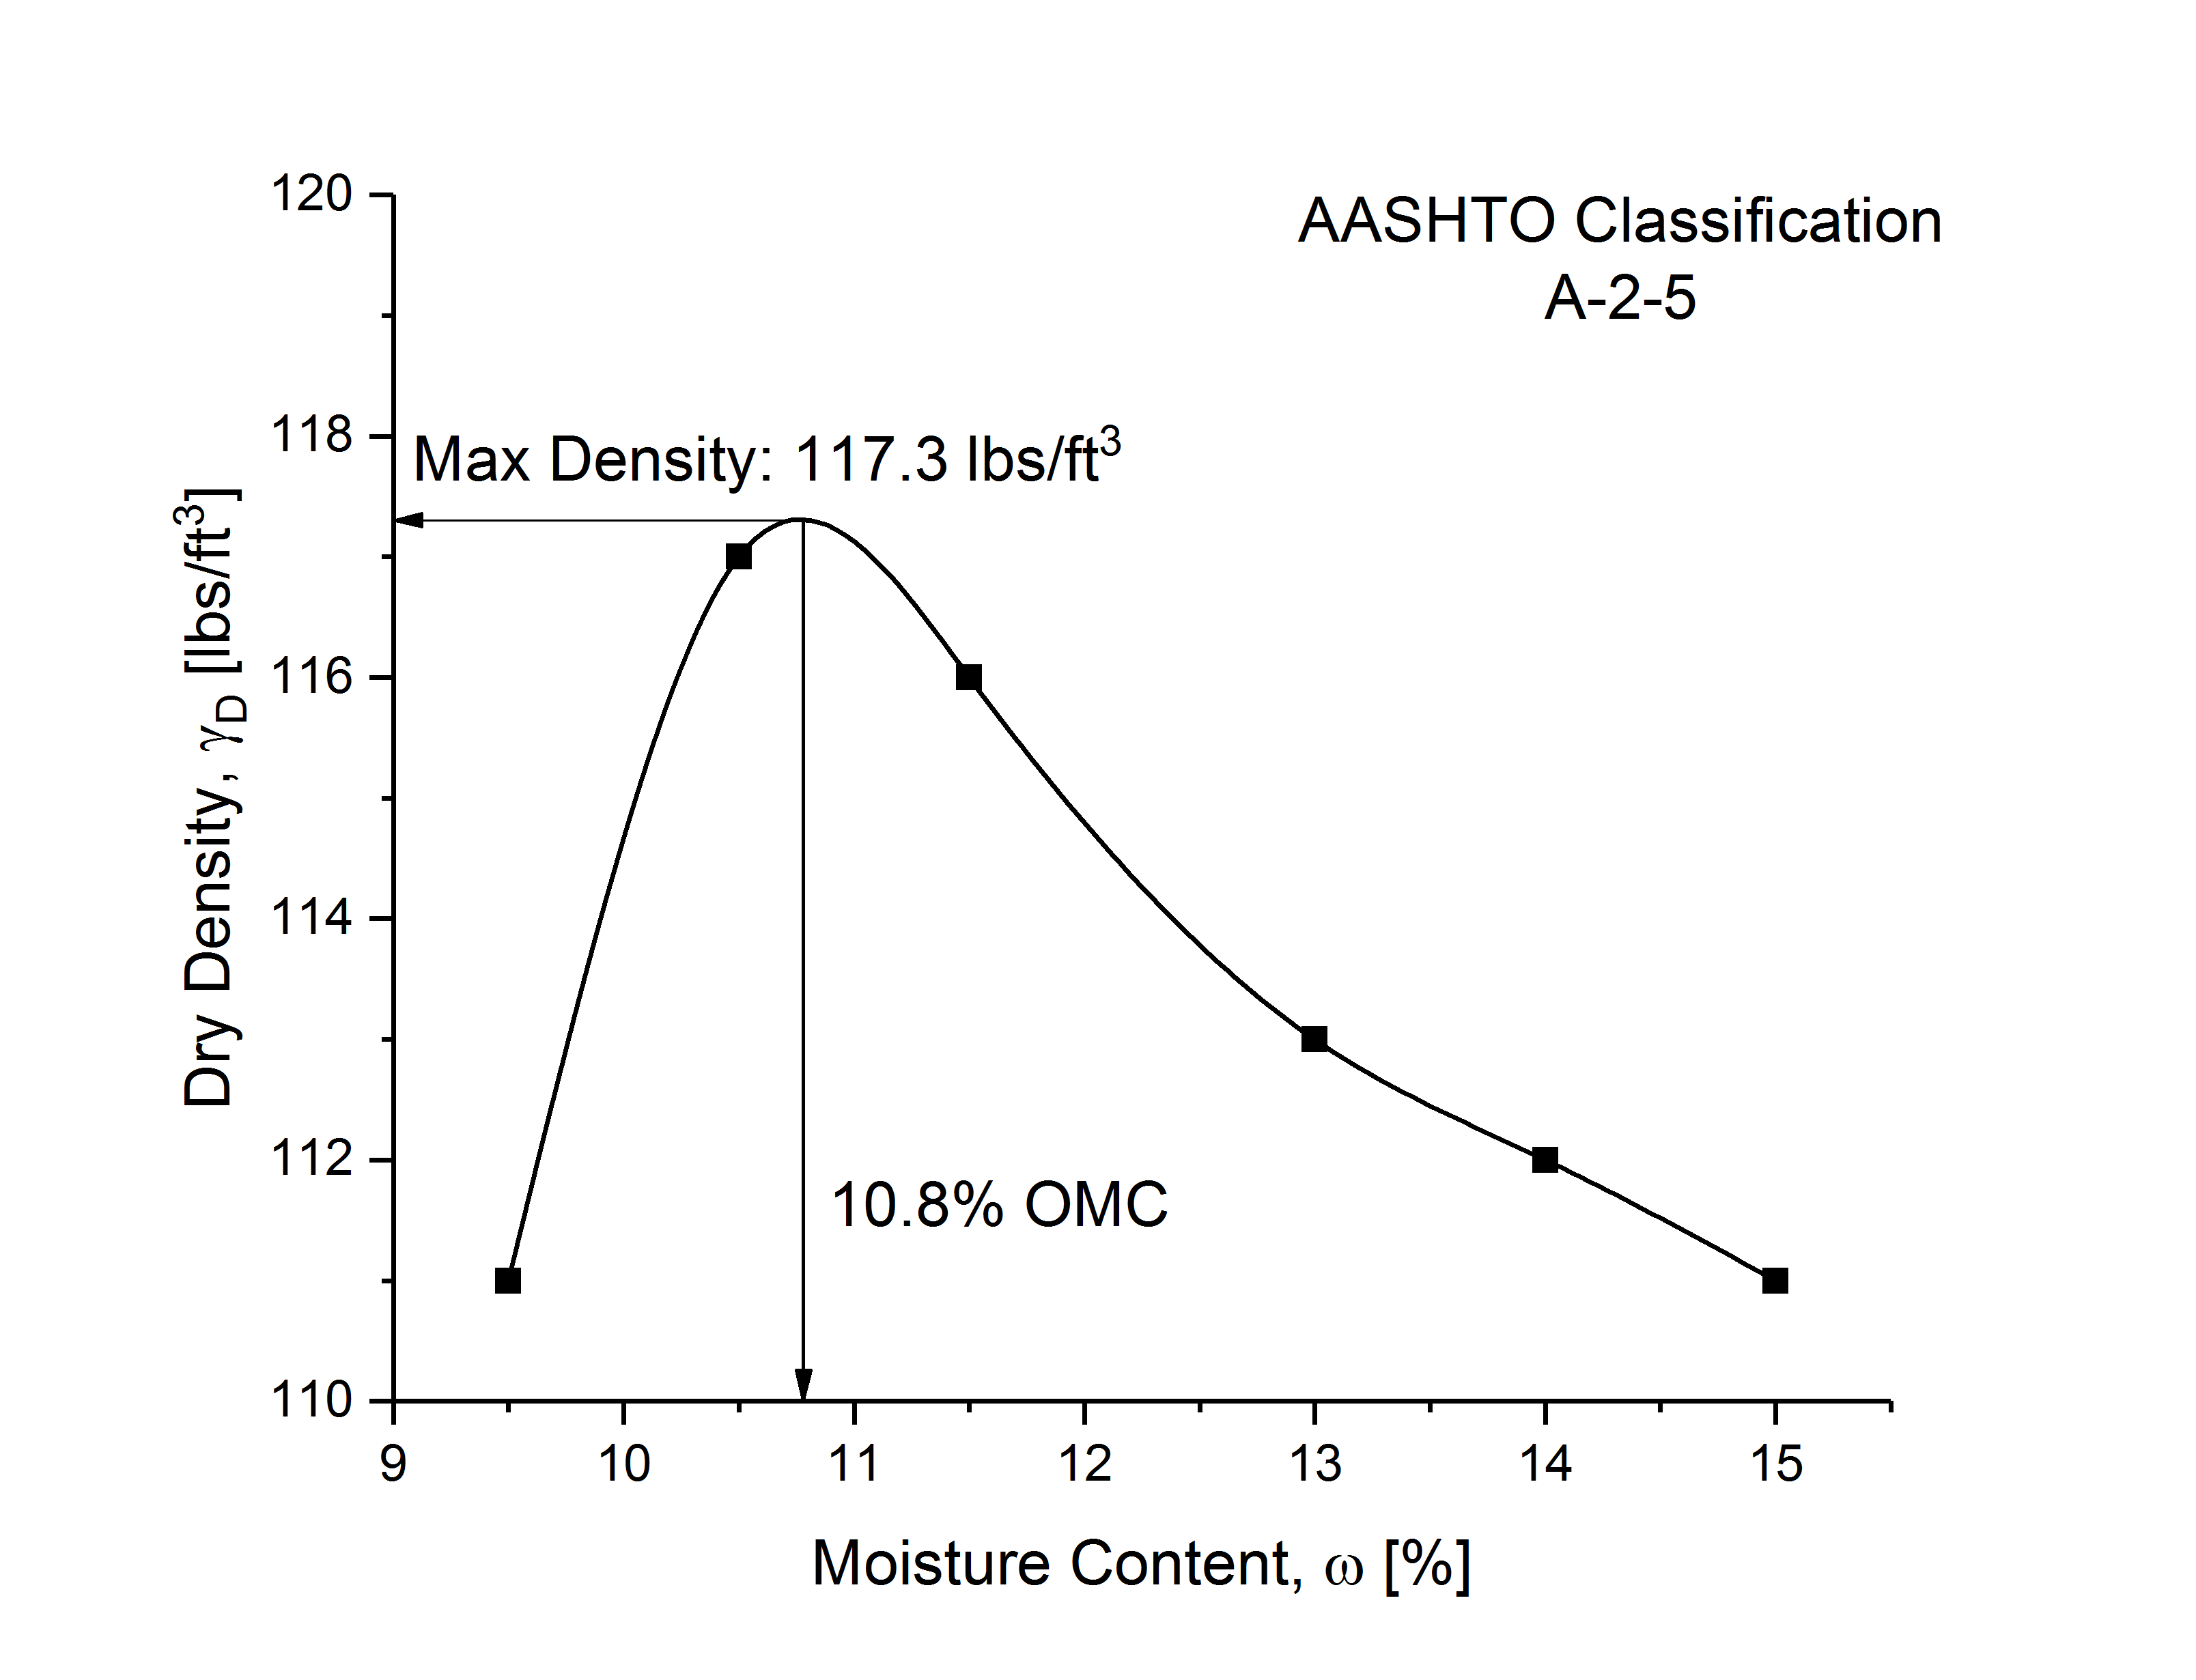
\includegraphics[width=0.7\textwidth]{exampleProctor.png}
\end{center}
\newpage
\question[10] Your boss, Hank Hill, is asking you for the dozer and scraper production time for each balance line shown in the mass-haul portion of the spreadsheet on Blackboard. Your scraper is a CAT 621F and your dozer is a CAT D8R (Semi-Universal Blade). For the dozer cases you have an average operator with a job efficiency of 40 min/hr dealing with a loose stockpile. For the scraper, use the chart below and read off of the 2\% resistance line.
\begin{center}
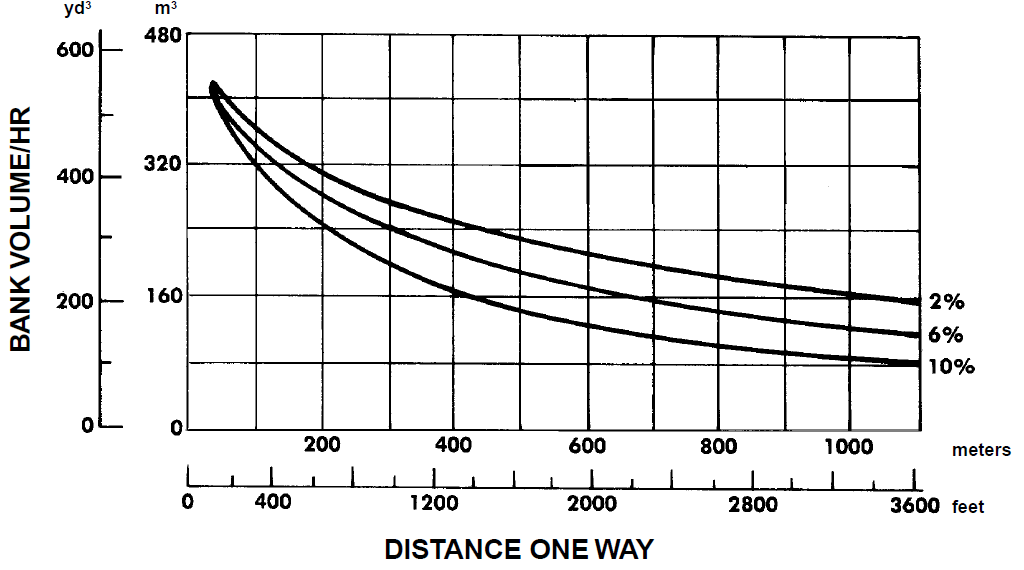
\includegraphics[width=0.8\textwidth]{scraper.png}\\
\small From: CAT Performance Handbook v. 29
\end{center}
Assuming there is only one dozer and one scraper for each balance line, how long will the earthwork take for each balance line? \textit{Hint: don't use the balance line distance, you need the average haul distance to get a much more realistic estimate!}
\question[6] Unfortunately, it got really hot during the earthwork phase in Q1 and after a new soil moisture survey, you need to figure out the compaction. Knowing that the current soil moisture content of the site is at 5.1\%, the width of the site is 30 ft, and the lift thickness is 7 inches, what is the water application rate needed, in gal/yd$^2$, to bring the moisture content to the OMC (determined in Q1) for both aggregate materials?
\newpage
\question[10] Now that the soil is all at OMC (OMG, amirite?), it's time to compact! This is another one of those open ended, no single correct answer questions that you know and love. Choose an appropriate compactor from the CAT Performance Handbook and calculate the time it will take to compact the entire site with just one compactor (to make calculations easier). Assume the site is completely flat and use any data needed from the previous questions to make your estimates. Couple of things to note:
\begin{itemize}
\item When determining the number of passes needed, you cannot use a value lower than the one assumed for the table (you can go higher if you want).
\item You may choose from either the single smooth drum rollers or the pneumatic tire rollers.
\item If you need to convert tons/hr to yd$^3$/hr, use the maximum dry density unit weight from Q1 to perform the calculation. Specify which aggregate source you are compacting.
\item You cannot use the double-drum or combi compactors.
\item You can travel up to the maximum speed of the equipment but not beyond. Each equipment has a different maximum speed.
\end{itemize}
\end{questions}

\begin{center}


\includegraphics[scale=0.6]{88x31.png}\\
This lecture exercise set by Dr. Armen N Amirkhanian is licensed under a Creative Commons Attribution-ShareAlike 4.0 International License.
\end{center}

The scraper production chart is from the freely available CAT Performance Handbook Volume 29 from Caterpillar.




\end{document}